\documentclass[10pt,twocolumn,letterpaper]{article}

\usepackage{times}
\usepackage{graphicx}
\usepackage{float}
\usepackage[italian]{babel}
\usepackage{csvsimple}
\usepackage[shortlabels]{enumitem}
\usepackage{listings}

\begin{document}


\title{Integral Image Generator\\
\large Parallel Programming for Machine Learning\\Project Work in Intelligent Systems}

\author{Sofia Galante\\
\small sofia.galante@stud.unifi.it\\
}
\date{}
\maketitle
\thispagestyle{empty}

\section{Introduzione}

Il progetto svolto è un generatore di immagini integrali.\\
In un’immagine integrale, partendo da un’immagine di partenza, un pixel è ottenuto sommando se stesso con tutti i pixel precedenti (sia lungo l’asse x che lungo l’asse y).\\
Si sono create tre diverse versioni di generatori di immagini integrali:
\begin{enumerate}
\item{un generatore sequenziale: in questo caso si generano le immagini integrali con un algoritmo sequenziale;}
\item{un generatore con CUDA: in questo caso si utilizza la GPU per parallelizzare la creazione dell’immagine integrale;}
\item{un generatore con OpenMP: in questo caso si compie una parallelizzazione a livello della CPU del codice tramite OpenMP.}
\end{enumerate}
Lo scopo del progetto è quello di osservare lo speedup ottenuto nelle due versioni parallele dell’algoritmo, osservando anche quale parallelizzazione (tra GPU e CPU) risulta più efficiente.\\
Tutti gli esperimenti sono stati svolti su un PC con sistema operativo Windows 10, una CPU intel i5 11400 e una GPU RTX 3070Ti.\\
La versione sequenziale e quella parallelizzata a livello di GPU utilizzando Visual C come compilatore, in quanto CUDA è compatibile solo con questo.\\
Per quanto riguarda la versione con OpenMP, si è optato per l’utilizzo di MinGW, in quanto Visual C dava problemi nell’annidare i cicli di parallel for.


\section{Organizzazione del codice}

Visto il costretto utilizzo di due compiler differenti, il codice è stato suddiviso in due diversi progetti (si è utilizzato CLion come IDE): un progetto che utilizza Visual C, e uno che utilizza MinGW. Inoltre un file .h è condiviso da entrambi i progetti.


\subsection{Il file condiviso: Image.h}

Il file condiviso da entrambi i progetti è il file \textbf{Image.h}, il quale contiene al suo interno la definizione di immagine, cioè una struct che ha come attributi una larghezza (width), un’altezza (height) e un puntatore di interi ad una locazione in memoria allocata dinamicamente (con malloc() se l’immagine è salvata nella CPU o con cudaMalloc() se è salvata sulla GPU).\\
\\
Questo file contiene anche una variabile globale (SEED), utilizzata come seed in entrambi i due progetti, così da generare le stesse immagini.


\subsection{I file del progetto con compiler Visual C}

Il primo progetto si occupa di allocare le immagini necessarie per i vari esperimenti e di salvarle in appositi file csv (utilizzando le funzioni condivise) così che si possano utilizzare le stesse immagini anche nel secondo progetto. Inoltre esso svolge i test di tipo sequenziale e di tipo parallelo su GPU e li salva in file csv.\\
I file presenti in questo progetto sono:

\begin{enumerate}
\item{ImageController.cuh/cu: i file che contengono la definizione e la dichiarazione di tutte le funzioni che si possono svolgere su un’Image. In particolare, si hanno funzioni per generare un’immagine casuale (generateImage()), funzioni per copiare un’immagine (copyImage()), funzioni per allocare/deallocare un’immagine dalla memoria (allocateImage(), freeHostImage(), freeDeviceImage()) e funzioni per copiare un’immagine sulla CPU dalla GPU e viceversa (copyFromDeviceToHost() e copyFromHostToDevice().}
\item{IntegralGeneratorSeq.cuh/cu: i file che contengono la definizione e la dichiarazione della funzione necessaria a svolgere l’algoritmo sequenziale (generateIntegralCPUseq());}
\item{IntegralGeneratorPar.cuh/cu: i file che contengono la definizione e la dichiarazione di due funzioni che implementano due diversi algoritmi paralleli con CUDA (generateIntegralGPUglobalMem() e generateIntegralGPUsharedMem()), una funzione che serve a calcolare la grandezza della grid e dei block in base alla dimensione dell'immagine da processare(findGridAndBlockDim()) e le funzioni di set up e fine, utilizzate per allocare, copiare e deallocare tutte le immagini necessarie su CPU e GPU; come detto sopra, si sono scritte due diverse implementazioni dell’algoritmo di tipo parallelo e, di questo, ne parleremo nel dettaglio nella sezione dedicata (la 3);}
\end{enumerate}


\subsection{I file del progetto con compiler MinGW}

Il secondo progetto si occupa di svolgere i test di tipo parallelo su CPU (con l’utilizzo di OpenMP) e di scrivere il risultato in un relativo file csv.\\
I file presenti in questo progetto sono:
\begin{enumerate}
\item{ImageController.h/cpp: questi file contengono le funzioni riguardanti le immagini salvate su CPU presenti in ImageController.cuh del primo progetto.}
\item{IntegralGeneratorOMP.h/cpp: i file che contengono al loro interno la dichiarazione e la definizione della funzione che svolge l’algoritmo parallelo con OpenMP (generateIntegralCPUomp()).}

\end{enumerate}


\section{Parallelizzazione con CUDA}
In IntegralGeneratorPar si trovano due diverse implementazioni dello stesso algoritmo parallelo.\\
\\
La prima di queste (NOME) è una parallelizzazione diretta della versione sequenziale dell’algoritmo: in questo caso ogni thread processa un singolo elemento dell’immagine e l’immagine originale e quella risultante si trovano entrambe nella memoria globale.\\
Questo tipo di algoritmo è penalizzato dai numerosi accessi alla memoria globale (uno ogni volta che si legge un elemento dell’immagine) che causano un aumento dell’effettivo tempo necessario.\\
\\
La seconda versione dell’algoritmo (NOME) utilizza la shared memory e la tecnica del tiling per risolvere il rallentamento dato dai continui accessi in global memory. La shared memory utilizzata viene allocata dinamicamente e dipende dalle dimensioni del blocco.\\
In questo algorimto, i thread di un blocco collaborano per caricare in shared memory gli elementi dell’immagine originale necessari per il calcolo. In particolare, l’algoritmo è stato diviso in fasi: ogni fase riguarda il caricamento di una quantità di elementi in shared memory pari alla grandezza di un block. Il numero di fasi di ogni block dipende dalla sua posizione nella grid: esso deve infatti caricare un numero di blocchi in memoria pari a tutti i blocchi con indice x o y precedente o uguale a sé.\\
Una volta caricati i blocchi in shared memory, i vari thread calcolano un valore provvisorio del risultato e, alla fine di tutte le fasi, ogni thread copia il valore calcolato nella giusta “casella” dell’immagine risultante.\\
\\
Si noti che per osservare un effettivo miglioramento nell’utilizzo del secondo algoritmo rispetto al primo si è dovuta disattivare manualmente attraverso il CMake la cache di primo livello: il compilatore infatti salvava nella cache gli elementi da leggere, rendendo il primo algoritmo veloce quanto (se non, in alcuni casi, più veloce) del secondo.


\section{Parallelizzazione con OpenMP}
La parallelizzazione dell’algoritmo svolta con l’utilizzo di OpenMP si trova in IntegralGeneratorOMP.\\
In questo caso, la parallelizzazione è stata effettuata con due diverse direttive \textit{parallel for}, annidate una dentro l'altra.\\
\\
La prima direttiva \textit{parallel for} (annidata a due livelli) parallelizza i due cicli for che danno le coordinate dell'elemento dell'immagine da calcolare.
\\
La seconda direttiva \textit{parallel for} (anche questa annidata a due livelli) parallelizza invece il calcolo dell'elemento selezionato in precedenza. Visto che il calcolo di ogni pixel deriva da una somma di tutti i pixel precedenti, per sfruttare al meglio le risorse di OpenMP si è deciso di utilizzare una \textit{reduction}.
\\
Si noti che la scrittura nell'immagine risultante non è stata marcata come sezione critica in quanto ogni thread modifica un diverso elemento dell'immagine, non causando quindi alcuna race condition.

\section{Esperimento svolto}
L'esperimento svolto in questo programma consiste nell'osservare lo speedup ottenuto dalle due parallelizzazioni su GPU e da quella su CPU a confronto con l’algoritmo sequenziale all’aumentare della dimensione dell’immagine.\\
\\
In questo esperimento si è variata la dimensione dell'immagine da 10x10 fino a 500x500, aumentando ogni volta sia l'altezza che la larghezza dell'immagine di 10 (quindi si sono svolte in totale 50 iterazioni).\\
Per questo grafico, vista l'enorme differenza tra i tempi di esecuzione, si è deciso di utilizzare una scala logaritmica lungo l'asse delle y.
\begin{figure}[H]
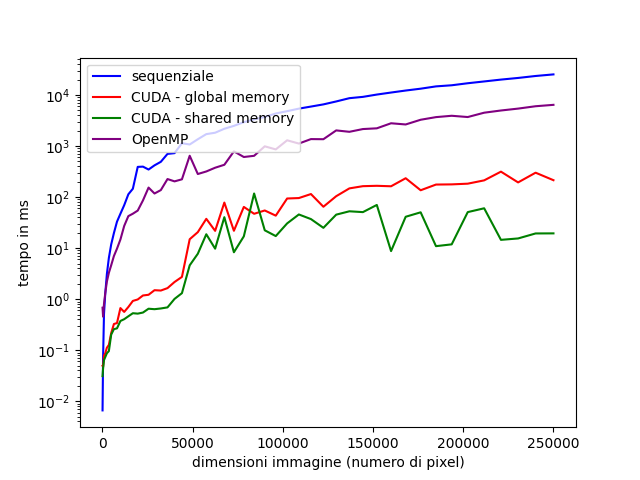
\includegraphics[width=1.1\linewidth]{test/test1} 
\caption{\small Tempo impiegato dall'esecuzione sequenziale e dalle tre esecuzioni parallele al variare della grandezza dell'immagine.}
\label{t1}
\end{figure}
Attraverso questo esperimento si può dunque notare come la versione parallelizzata attraverso CUDA sia molto più veloce non solo della versione sequenziale ma anche della versione parallelizzata attraverso OpenMP. Questo prova come la parallelizzazione compiuta attraverso la GPU sia superiore di quella compiuta attraverso la CPU.\\
Si noti inoltre come la versione che utilizza la \textbf{shared memory} sia più veloce di quella che invece utilizza la \textbf{global memory} e questa differenza dei tempi aumenta (salvo delle eccezioni) con l'aumentare dell'immagine di partenza.\\
\\
Un'ulteriore osservazione che è possibile fare è però il fatto che, mentre i tempi di esecuzione dei due algoritmi su CPU tendono a aumentare con l'aumentare della dimensione dell'immagine, per quanto riguarda i due algoritmi della GPU questo non è completamente vero: in questo caso i tempi tendono a oscillare.\\
Questo fatto deriva da come viene divisa l'immagine tra i diversi blocchi della GPU.

\end{document}